\section{Electro-Pneumatic System\label{sec:electropneumatic_implementation}}

\nomenclature{PID}{Proportional-Integral-Differential}

Several steps were taken in the implementation phase to develop a better understanding of the electro-pneumatic's behaviour, and to provide data and models that could be used in the implementation of the controller software. A Simulink model was developed to verify that our fundamental design would work, and to gain further insight into the operation of the electro-pneumatic system. A simple \emph{Proportional-Integral-Derivative} (PID) controller block was used to show that the closed-loop system was inherently stable.

\subsection{Simulation with Simulink}

An overview of the Simulink model used to simulate the electro-pneumatics system is shown in \ref{fig:pneumatics_top_level}. A PID controller block is used in a closed-loop configuration, and the response to a fixed step input is displayed on the scope block. 

\begin{figure}[H]
\centering
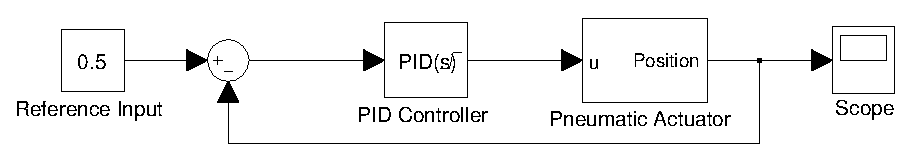
\includegraphics[scale=1]{implementation/figures/pneumatic_modelling1.eps}
\caption{Simulink model of the electro-pneumatic system.}
\label{fig:pneumatics_top_level}
\end{figure}

The three major components of the electro-pneumatic system are the \emph{PWM generator}, the \emph{solenoid valves}, and the \emph{pneumatic actuator}. Models of these systems are described further in the following sections.

\subsubsection{PWM Generator Model}

The PWM generator is used to provide the electrical control signals required by the solenoid valves to open and close. Our model of the PWM generator uses the instantaneous model presented by \citet{valve_models}. This model compares a generated saw-tooth signal $V_{saw}$ with the input signal $V_{in}$ over a time period $T_{saw}$ to obtain the pulse-width-modulated signal $U(t)$. The relationship is illustrated in Eq. \ref{eq:pwm_generation}.

\begin{equation}
\label{eq:pwm_generation}
U\left(t\right) = 
\begin{cases}
1 & V_{in}\left(t\right) \geq V_{saw}\left(t\right) \\
0 & V_{in}\left(t\right) < \left(t\right)
\end{cases}
\end{equation}

The Simulink model which implements Eq. \ref{eq:pwm_generation} can be seen in Fig.\ \ref{fig:pneumatics_pwm}. The input to the subsystem, shown as \emph{In1}, is $V_{in}$, and the output, shown as \emph{Out1} is the pulse width modulated signal $U(t)$. 

\begin{figure}[H]
\centering
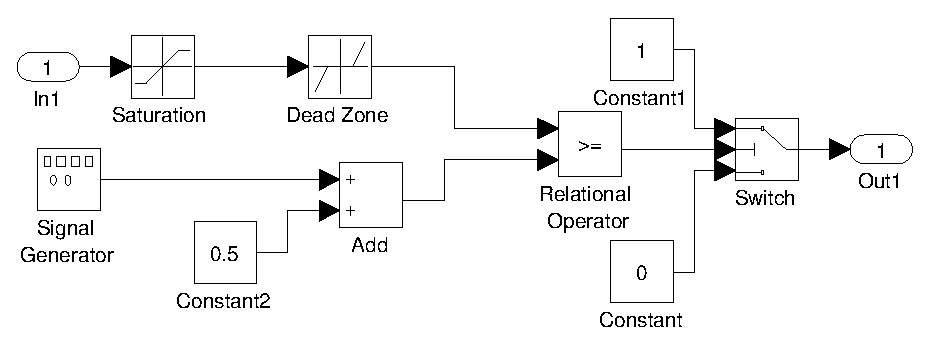
\includegraphics[scale=0.65]{implementation/figures/pneumatic_modelling2.eps}
\caption{Simulink model of the PWM generator.}
\label{fig:pneumatics_pwm}
\end{figure}

A saturation block limits the input signal $V_{in}$ to the range of \unit{[0..1]}{\volt}. A dead-zone block is present to account for the dead-zone present in the solenoid valve response to a PWM signal. If the pulse width is too short, the current through the solenoid cannot generate enough force to open the poppet, so the valve stays shut. This is a parameter of the solenoid valve, and was quantified experimentally by \cite{valve_models} as the minimum input signal $V_{in}$ required to open the valve. \Citet{accurate_position} also account for a minimum possible duty cycle in the solenoid valve input signal, known as $d_{min}$. This value can be calculated as:

\begin{equation}
  \label{eq:pwm_duty_min}
  d_{min}=\left(T_{vr}/T_{PWM}\right)\cdot100\%
\end{equation}

In this case, $T_{vr}$ is the time required by a solenoid valve to respond to an input, and $T_{PWM}$ the period of the PWM signal.

\nomenclature{$d_{min}$}{The minimum possible duty cycle of a solenoid's drive signal that will cause the valve to open.}
\nomenclature{$T_{vr}$}{The time required by a solenoid valve to respond to an input.}

The signal generator block in Fig.\ \ref{fig:pneumatics_pwm} outputs a triangle wave with peak-to-peak amplitude of \unit{1}{\volt}, which is then offset by \unit{0.5}{\volt}. The relational operator block then compares this with the input signal, and outputs the resulting PWM signal.

\subsubsection{Solenoid Valve Model}

An initial Simulink model of a solenoid valve was constructed based on the modelling equations described by \citet{valve_models} and the standard orifice equations for laminar and choked flow described in \cite{fluid_power}. However, it was too difficult to identify the system parameters cited in \cite{fluid_power} for our specific solenoid valves. The solenoid's data-sheet was not detailed enough, and the straight-forward approach to system identification used by \cite{valve_models} required specialized measuring equipment (such as an instantaneous mass flow meter) that we did not have access to.

\subsubsection{Pneumatic Actuator Model}

Simulink's pneumatic actuator subsystem is illustrated in Fig.\ \ref{fig:pneumatics_actuator}. Pre-built Simulink blocks from the Simscape package were used to model the dynamics of the actuator. \emph{Physical Port 1} (denoted by the octagonal port symbol with a ``1'' inside) in \ref{fig:pneumatics_actuator} represents the air inlet. \emph{Physical Ports 2 and 3} (denoted by the octagonal port symbols with a ``2'' and ``3'' inside, respectively) represent the displacement ports of the cylinder. \emph{Regular Port 1} (denoted by the rounded port symbol with a ``1'' inside) is used to display the displacement on a scope.

\begin{figure}[H]
\centering
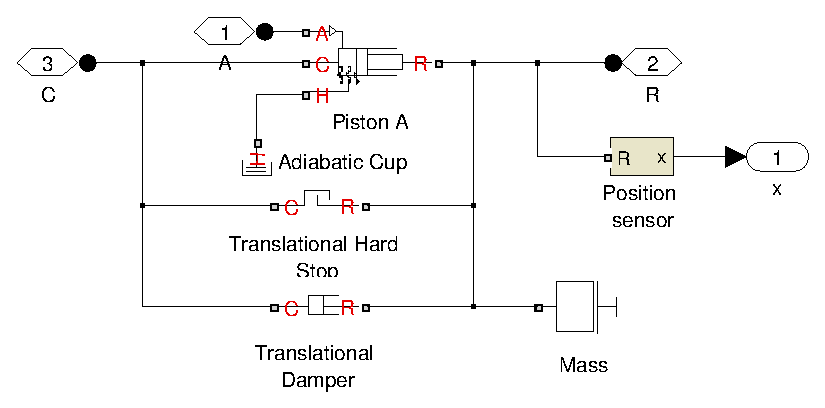
\includegraphics[scale=0.65]{implementation/figures/pneumatic_modelling3}
\caption{Simulink model of the pneumatic actuator.}
\label{fig:pneumatics_actuator}
\end{figure}

\subsubsection{Integrated Simulink Model}

The complete open-loop actuator model can be seen in Fig.\ \ref{fig:pneumatics_model_full}. The absolute value of the real-valued input $u$ is first fed to the PWM block. This signal is then converted into separate signals for each of the two solenoid valves in a way similar to the first PWM pulsing scheme presented by \citet{accurate_position}. The input to the subsystem $u$ is expected to range from -1 to 1. When $u\geq0$, the input to valve A is the pulse width modulated signal $U$, and the input to valve B is 0. When $u<0$, the opposite situation occurs.

\begin{figure}[H]
\centering
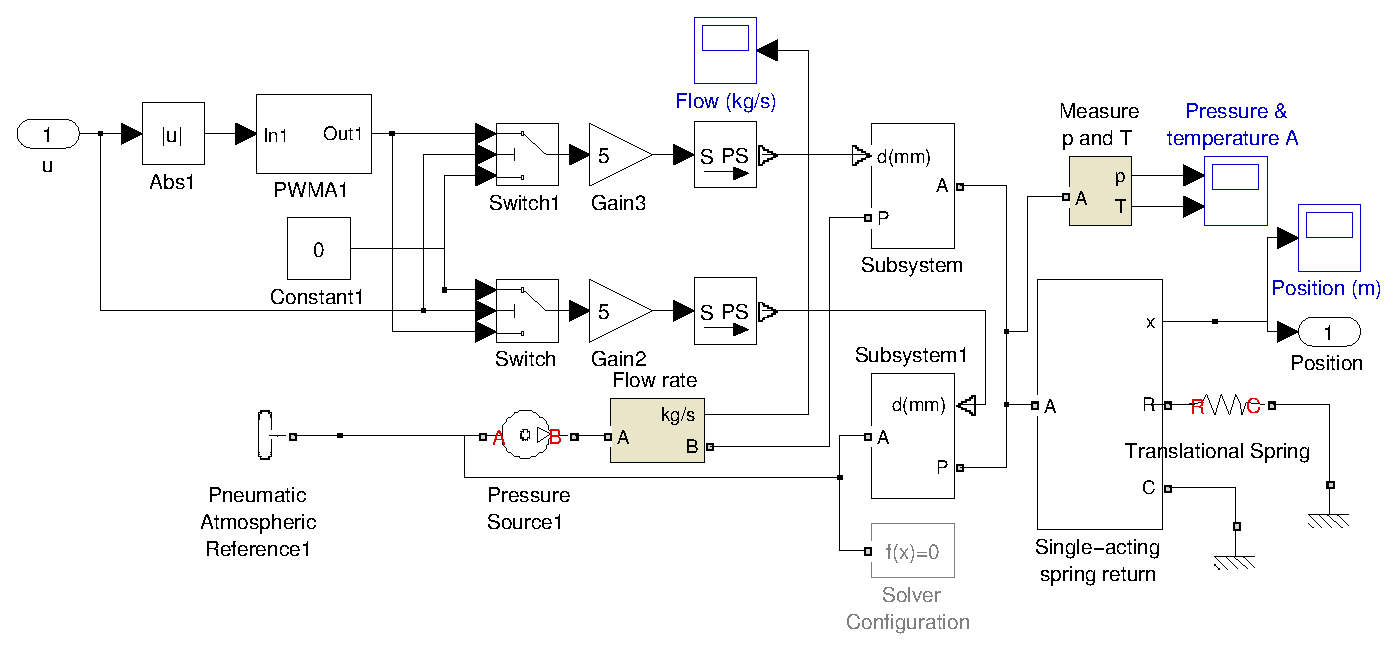
\includegraphics[scale=0.65]{implementation/figures/pneumatic_modelling4}
\caption{Simulink model of the full electro-pneumatic system.}
\label{fig:pneumatics_model_full}
\end{figure}

\subsection{Component Selection}

Selection of components was limited by budgetary constraints, however adequate solenoid valves and pneumatic actuators were found. These are detailed in the following sections.

\subsubsection{Solenoid Valves}

Solenoid valves and cylinders from SMC corp were chosen for the physical implementation of the design, specifically the \emph{VQZ115} series valve. Table \ref{tab:solenoid_specs} shows the specifications for this solenoid valve. A maximum operating frequency of \unit{20}{\hertz} was the fastest available solenoid that met the output force requirements while still being within the Formula SAE budget.

\begin{table}[H]
  \caption{Specifications of the SMC VQZ115 solenoid valve.\label{tab:solenoid_specs}}
  \centering

  \begin{tabular}{|l|l|}
  \hline 
  Part & VQZ115-6L1-N1-PR \tabularnewline
  \hline
  \hline
  Coil Voltage & \unit{12}{\volt} \tabularnewline
  \hline
  Configuration & 3-port Normally Closed \tabularnewline
  \hline
  Flow Coefficient & $C_v=\unit{0.23}{}$ \tabularnewline
  \hline
  Maximum Operating Frequency & \unit{20}{\hertz} \tabularnewline
  \hline
  Maximum Pressure & \unit{0.7}{\mega\pascal} \tabularnewline
  \hline
  \end{tabular}
\end{table}

\subsubsection{Pneumatic Actuators}

The pneumatic actuators specified for implementation are the same as used in the previous design, and are only briefly mentioned in this report. Specifications can be found in Table \ref{tab:cylinder_specs}. The clutch cylinder is specified with an internal magnet on the piston that interfaces magnetically with a membrane potentiometer.

\begin{table}[H]
 \caption{Specifications of the pneumatic actuators used.\label{tab:cylinder_specs}}
  \centering
  \begin{tabular}{|l|l|l|l|}
   \hline
   Part & Bore Size & Stroke & Part Number \tabularnewline
    \hline
    \hline
    Shift actuator & 9/16`` & 2'' & NCMC056-0200 \tabularnewline
    \hline
    Clutch actuator & 3/4`` & 2'' & NCDMC075-0200 \tabularnewline
    \hline
  \end{tabular}
\end{table}

\subsubsection{Positional Feedback Sensors}

A ``MagnetoPot'' contact-less potentiometer from Spectra Symbal provides positional feedback from the clutch cylinder. The internal magnet in the cylinder interacts with the ``MagnetoPot'', which has a three-wire electrical interface similar to a standard potentiometer.
